\section{Figuras e tabelas}
%------------------------------------------
%----------------FIGURE--------------------
\begin{figure*}[ht!]
\centering
\includegraphics[width = 11 cm]{figuras/Gráfico F^2.png}
\caption{\small{Linearização e ajuste linear dos dados para correntes positivas e negativas. Barras de incerteza pontuais não são visíveis devido à escala, porém foram consideradas pelo programa na obtenção dos coeficientes.}}
\label{fig:1}
\end{figure*}

\begin{figure*}[ht!]
\centering
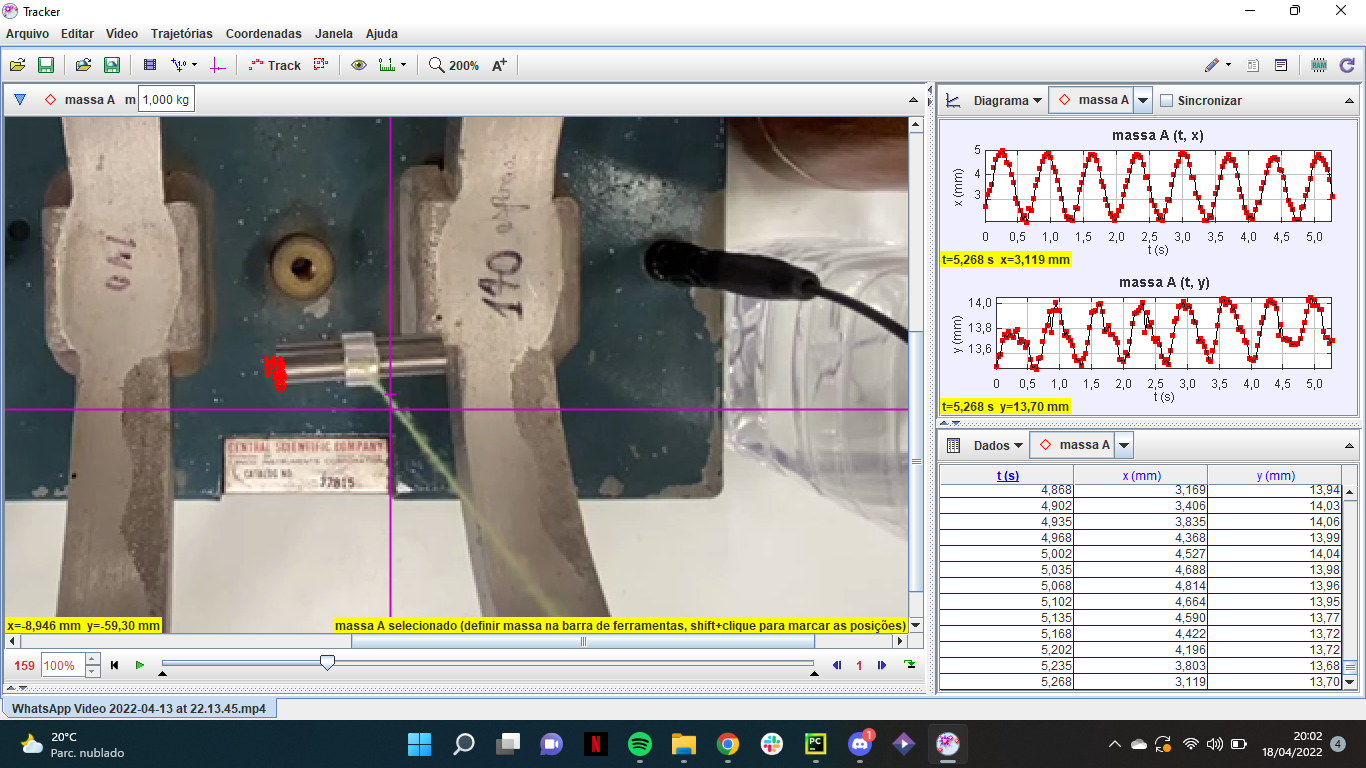
\includegraphics[width = 11 cm]{figuras/Captura de Tela (78).png}
\caption{\small{Obtenção da frequência pelo Tracker.}}
\label{fig:1}
\end{figure*}
%------------------------------------------
%------------------------------------------


%------------------------------------------
%----------------FIGURE--------------------
%------------------------------------------
%------------------------------------------

\begin{table}[ht!]
\center
\begin{tabular}{|l|l|l|}
\hline
 & $\mu$ (J/T)& $B_t$  ($\mu$T)\\ \hline
Corrente positiva &$(2.14 \pm 0.02) \times 10^{-1}$& 18$\pm$2 \\ \hline
Corrente negativa &$(-1.98 \pm 0.07) \times 10^{-1}$ & $4 \pm 6$ 
\\ \hline
\end{tabular}
\caption{Valores de $\mu$ e $B_t$ para cada reta.}
\label{tab:1}
\end{table}

Dados coletados podem ser vistos em: \url{https://docs.google.com/spreadsheets/d/1FT3ynu-3OVvudksDfkpWPYaOrA59bLVI8ZYq9izyZq8/edit#gid=0}.
%------------------------------------------
%------------------------------------------

